\documentclass[11pt]{book}
\usepackage{hyperref}
\usepackage{amsfonts}
\usepackage{amssymb}
\usepackage{amsmath}
\usepackage[utf8]{inputenc}
\usepackage[T1]{fontenc}
\usepackage{float}
\usepackage{fixltx2e}
\usepackage[italian]{babel}
\usepackage{graphicx}

\newenvironment{sistema}%
{\left\lbrace\begin{array}{@{}l@{}}}%
{\end{array}\right.}


\title{Appunti di Ricerca Operativa}
\author{Fabio Viola}
\date{}

\hyphenation{mi-ni-miz-za-re}

\setcounter{chapter}{3}

\begin{document}

\chapter{L'algoritmo del simplesso}

\scriptsize
{\bf Slide}:
\href{http://www.or.deis.unibo.it/staff_pages/martello/Chapter4.zip}{The
Simplex Algorithm}
\normalsize
\vspace{20pt}

\section{Strategia generale}

Riassumiamo quanto abbiamo studiato fin'ora. Vogliamo {\bf
  minimizzare} la {\bf funzione obiettivo} $c'x$ con $x \in F = \{ x
\in \mathbb{R}^n : Ax = b, x \geq 0 \}$ assumendo che il rango di {\em
  A} sia {\em m} e che l'insieme delle soluzioni {\em F} sia non vuoto
e limitato nella direzione di decrescita della funzione
obiettivo. Tali assunzioni dovranno poi essere verificate
dall'algoritmo. All'interno della matrice {\em A} \`e possibile
individuare un insieme di {\bf colonne linearmente indipendenti} che
chiamiamo {\bf base} e indichiamo con $\mathcal{B}$. Ad essa
corrisponder\`a la matrice {\em B}. Ponendo a 0 le {\em x}
corrispondenti alle colonne fuori base e risolvendo il sistema
$Bx_\beta = b$ (dove $x_\beta$ \`e un vettore composto dalle {\em
  variabili in base}) si ottiene una soluzione che chiamiamo {\bf
  soluzione di base}. Se $x \geq 0$ in ogni sua componente allora
questa \`e detta {\bf soluzione di base ammissibile} ({\em BFS} o {\em
  SBA}). Tale soluzione individua un vertice del politopo. Una delle
{\em SBA} fornisce sicuramente la soluzione ottima e dunque la nostra
ricerca si concentrer\`a proprio sulle {\em SBA}. Introduciamo una
definizione che ci servir\`a per spiegare la strategia seguita dal
metodo del simplesso: date due {\em SBA} distinte, queste si dicono
{\bf adiacenti} se differiscono per una sola colonna (formalmente
diciamo che due {\em SBA} distinte appartenenti a due basi
$\mathcal{B}$ e $\bar{\mathcal{B}}$ sono adiacenti se $\exists A_j \in
\mathcal{B},\phantom{a}A_k \in
\bar{\mathcal{B}}\phantom{a}:\phantom{a}\bar{\mathcal{B}} =
(\mathcal{B} \textbackslash \{ A_j \}) \cup \{ A_k \}$). L'{\bf
  algoritmo del simplesso} sfrutta la seguente strategia:

\begin{quote}
{\em Partendo da una {\em SBA} qualunque, iterativamente si sostituisce la
{\em SBA} corrente con una adiacente di costo non maggiore, fino a
trovare la {\em SBA} ottima.}
\end{quote}

\section{Spostamento da una SBA ad un'altra}

Come abbiamo visto, spostarsi da una {\em SBA} ad un'altra \`e la base
dell'algoritmo del simplesso dunque vediamo il procedimento algebrico
necessario.

Prendiamo una base $\mathcal{B} = \{ A_{\beta(i)} : i = 1, \dots, m
\}$; indichiamo con $x_0$ la {\em SBA} corrispondente e in particolare
chiamiamo $y_{i0}$ con $i = 1, \dots, m$ le componenti di base. Il
vettore $x_0$ si pu\`o scrivere come (trascurando l'ordine delle
componenti):

\begin{center}
\begin{equation}
x_0' = (y_{10}, y_{20}, \dots, y_{m0}, 0, \dots, 0) \geq 0
\end{equation}
\end{center}

Dato che vale $Ax_0 = b$, possiamo scrivere:

\begin{center}
\begin{equation}
\sum\limits_{i=1}^m y_{i0} A_{\beta(i)} = b
\label{prima}
\end{equation}
\end{center}

Dal momento che le colonne della base sono linearmente indipendenti
possiamo esprimere una qualunque altra colonna $A_j$ fuori base come una
combinazione lineare delle colonne $A_{\beta(i)}$. Esisteranno dunque
dei coefficienti $y_{ij}$ tali che:

\begin{center}
\begin{equation}
\sum\limits_{i=1}^m y_{ij} A_{\beta(i)} = A_j
\label{seconda}
\end{equation}
\end{center}

Moltiplicata per uno scalare $\vartheta$ diventa:

\begin{center}
\begin{equation}
\sum\limits_{i=1}^m \vartheta y_{ij} A_{\beta(i)} = \vartheta A_j
\label{terza}
\end{equation}
\end{center}

Effettuando la sottrazione fra la prima sommatoria introdotta e la
precedente otteniamo:

\begin{center}
\begin{equation}
\sum\limits_{i=1}^m y_{i0} A_{\beta(i)} - \vartheta y_{ij} A_{\beta(i)} +
  \vartheta A_j = \sum\limits_{i=1}^m (y_{i0} - \vartheta y_{ij})
  A_{\beta(i)} + \vartheta A_j = b\phantom{aaa}\forall A_j \not\in
  \mathcal{B}
\label{theta}
\end{equation}
\end{center}

Il tutto sar\`a pi\`u chiaro a breve con un esempio.

Assumiamo per il momento che $x_0$ {\bf non} sia degenere, cio\`e che
$y_{10} > 0 \forall i$. Osserviamo che porre $\vartheta = 0$ significa
considerare l'equazione \ref{prima}, cio\`e trovare la {\em SBA} della
base {\em B}. All'aumentare di $\vartheta$ troviamo invece nuove
soluzioni ammissibili, questa volta con m+1 componenti positive
(ancora una volta rimandiamo all'esempio per maggior
chiarezza). $\vartheta$ non pu\`o assumere indiscriminatamente
qualsiasi valore, ma sar\`a limitato. Il massimo valore che
$\vartheta$ pu\`o assumere per il problema di {\em LP} \`e quello in
cui il primo coefficiente di \ref{theta} diventa 0. Se aumentassimo
ulteriormente $\vartheta$ avremmo un valore negativo e violeremmo il
vincolo $x \geq 0$. Ecco dunque che $\vartheta$ pu\`o assumere al
massimo il valore:

\begin{center}
\begin{equation}
\vartheta_{max} = \underset{i:y_{ij}>0}{min} \frac{y_{i0}}{y_{ij}}
\label{thetamax}
\end{equation}
\end{center}

Quando $\vartheta$ asume tale valore, la relazione \ref{theta} esprime
nuovamente una soluzione con $m$ componenti positive. In questa nuova
soluzione viene inclusa la colonna $A_j$, ma non quella in cui il
coeffciente si \`e azzerato permettendo di tornare da $m+1$ componenti
a $m$.\newline\vspace{11pt}

$\blacktriangleright$ {\bf Esempio} \dots

\begin{center}
\[
A = 
\begin{bmatrix}
1 & 1 & 1 & 1 & 0 & 0 & 0 \\
1 & 0 & 0 & 0 & 1 & 0 & 0 \\
0 & 0 & 1 & 0 & 0 & 1 & 0 \\
0 & 3 & 1 & 0 & 0 & 0 & 1
\end{bmatrix},
b = 
\begin{bmatrix}
4 \\ 2 \\ 3 \\ 6
\end{bmatrix}
\],
\end{center}

Prendiamo come base $\mathcal{B} = \{ A_1, A_3, A_6, A_7\}$. Questo
vuol dire che gli indici di base sono: $\beta(1) = 1, \beta(2) = 3,
\beta(3) = 6, \beta(4) = 7$. 

\begin{center}
\[
y_{10} \cdot
\begin{bmatrix}
1 \\ 1 \\ 0 \\ 0
\end{bmatrix}
+ y_{20} \cdot
\begin{bmatrix}
1 \\ 0 \\ 1 \\ 1
\end{bmatrix}
+ y_{30} \cdot
\begin{bmatrix}
0 \\ 0 \\ 1 \\ 0
\end{bmatrix}
+ y_{40} \cdot
\begin{bmatrix}
0 \\ 0 \\ 0 \\ 1
\end{bmatrix}
= 
\begin{bmatrix}
4 \\ 2 \\ 3 \\ 6
\end{bmatrix}
\]  
\end{center}

Da cui scaturisce il sistema:

\begin{center}
$\begin{sistema}
y_{10}\cdot 1 + y_{20}\cdot 1 + y_{30}\cdot 0 + y_{40}\cdot 0  = 4 \\
y_{10}\cdot 1 + y_{20}\cdot 0 + y_{30}\cdot 0 + y_{40}\cdot 0  = 2 \\
y_{10}\cdot 0 + y_{20}\cdot 1 + y_{30}\cdot 1 + y_{40}\cdot 0  = 3 \\
y_{10}\cdot 0 + y_{20}\cdot 1 + y_{30}\cdot 0 + y_{40}\cdot 1  = 6 \\
\end{sistema}
=
\begin{sistema}
y_{10} + y_{20} = 4 \\
y_{10} = 2 \\
y_{20} + y_{30}  = 3 \\
y_{20} + y_{40} = 6 \\
\end{sistema}
$
\end{center}

Otteniamo che la soluzione di base ammissibile per questa base \`e:

\begin{center}
$x_0 = (2, 0, 2, 0, 0, 1, 4)$  
\end{center}

dove 2, 2, 1 e 4 corrispondono rispettivamente a $y_{10}$, $y_{20}$,
$y_{30}$, $y_{40}$.

A questo punto scegliamo una variabile fuori base $j=5$. Per quanto
affermato potremo scrivere:

\begin{center}
$A_5 = \sum\limits_{i=1}^m y_{i5}A_i = y_{15} \cdot A_1 + y_{25} \cdot
  A_2 + y_{35} \cdot A_3 + y_{45} \cdot A_4 $
\end{center}

cio\`e:
\begin{center}
\[
y_{15} \cdot
\begin{bmatrix}
1 \\ 1 \\ 0 \\ 0
\end{bmatrix}
+ y_{25} \cdot
\begin{bmatrix}
1 \\ 0 \\ 1 \\ 1
\end{bmatrix}
+ y_{35} \cdot
\begin{bmatrix}
0 \\ 0 \\ 1 \\ 0
\end{bmatrix}
+ y_{45} \cdot
\begin{bmatrix}
0 \\ 0 \\ 0 \\ 1
\end{bmatrix}
= 
\begin{bmatrix}
0 \\ 1 \\ 0 \\ 0
\end{bmatrix}
\]  
\end{center}

e otteniamo i coefficienti $y_{i5}$: $1, -1, 1, 1$. In questo modo
abbiamo trovato i coefficienti che ci permettono di esprimere $A_5$
come combinazione lineare delle colonne della base $B$. Adesso
proviamo a trovare una nuova base.

Applichiamo \ref{theta} ed otteniamo:

\begin{center}
\[
(2-\vartheta) \cdot A_1 + (2+\vartheta) \cdot A_3 + (1-\vartheta)
\cdot A_6 + (4-\vartheta) \cdot A_7 + \vartheta \cdot A_7 = b
\]
\end{center}

pi\`u esplicitamente:

\begin{center}
\[
(2-\vartheta) \cdot
\begin{bmatrix}
1 \\ 1 \\ 0 \\ 0
\end{bmatrix}
+ (2+\vartheta) \cdot
\begin{bmatrix}
1 \\ 0 \\ 1 \\ 1
\end{bmatrix}
+ (1-\vartheta) \cdot
\begin{bmatrix}
0 \\ 0 \\ 1 \\ 0
\end{bmatrix}
+ (4-\vartheta) \cdot
\begin{bmatrix}
0 \\ 0 \\ 0 \\ 1
\end{bmatrix}
+ \vartheta \cdot
\begin{bmatrix}
0 \\ 1 \\ 0 \\ 0
\end{bmatrix}
= 
\begin{bmatrix}
4 \\ 2 \\ 3 \\ 6
\end{bmatrix}
\]  
\end{center}

Quest'equazione descrive la famiglia di punti $(2-\vartheta, 0,
2+\vartheta, 0, \vartheta, 1-\vartheta, 4-\vartheta) \in
\mathbb{R}^7$.

Troviamo $\vartheta_{max}$: 

\begin{center}
\[
\vartheta_{max} =
min \biggr\{ \frac{2}{1},-\frac{2}{1},\frac{1}{1},\frac{4}{1} \biggr\}
=
min \biggr\{ \frac{2}{1},\frac{1}{1},\frac{4}{1} \biggr\}  = 1
\]
\end{center}

Sostituiamo dunque 1 a $\vartheta$ e ci spostiamo in questo modo da
$x_0$ a $\tilde{x}_0 = (1, 0, 3, 0, 1, 0, 3)$. A questo corrisponde il
nuovo insieme di colonne $\mathcal{\tilde{B}} = \{ A_1, A_3, A_5,
A_7\}$. Come possiamo vedere \`e uscita dalla base la colonna 6 per
lasciare il posto alla colonna 5. Spostarsi dal vertice $x_0$ al nuovo
vertice $\tilde{x}_0$ corrisponde a muoversi lungo il segmento che li
unisce e prendere un $\vartheta$ maggiore di $\vartheta_{max}$
porterebbe ad uscire dal politopo. $\blacktriangleleft$
\newline
\vspace{11pt}

Abbiamo assunto che $x_0$ non fosse degenere. Vediamo cosa succede
invece se lo \`e. Se $x_0$ \`e degenere esiste almeno un $i'$ tale per
cui $y_{i'0} = 0$. Se nel momento in cui si vuole esprimere una
colonna $A_j$ come combinazione lineare della base che ci ha permesso
di trovare $x_0$ trovassimo un coefficiente $y_{i'j}$ positivo in
\ref{theta}, allora avremmo $\vartheta_{max} = 0$ e quindi la nuova
soluzione $\tilde{x}_0$ sarebbe identica a $x_0$ pur variando
l'insieme delle colonne.

Abbiamo inoltre assunto che $\vartheta_{max}$ potesse essere calcolato
con \ref{thetamax}, ma ci\`o non \`e sempre vero se si hanno tutti i
coefficienti $y_{ij} \leq 0$. In questo caso, basta osservare
l'equazione \ref{theta}, il valore di $\vartheta_{max}$ pu\`o crescere
illimitatamente senza violare l'ammissibilit\`a delle
soluzioni. Questo implica che possiamo spostarci all'interno del
politopo senza uscirne mai, ergo il politopo \`e illimitato (ci\`o
viola una delle assunzioni fatte nel precedente capitolo). In questo
caso la soluzione tende a $-\infty$.

\section{Il tableau e il pivoting}

Il {\bf tableau} \`e lo strumento fondamentale per eseguire con
semplicit\`a il cambiamento di base. Il tableau \`e una
rappresentazione compatta del sistema $Ax=b$, nella forma visibile in
figura \ref{tableau}.

\begin{figure}[h!]
  \centering
  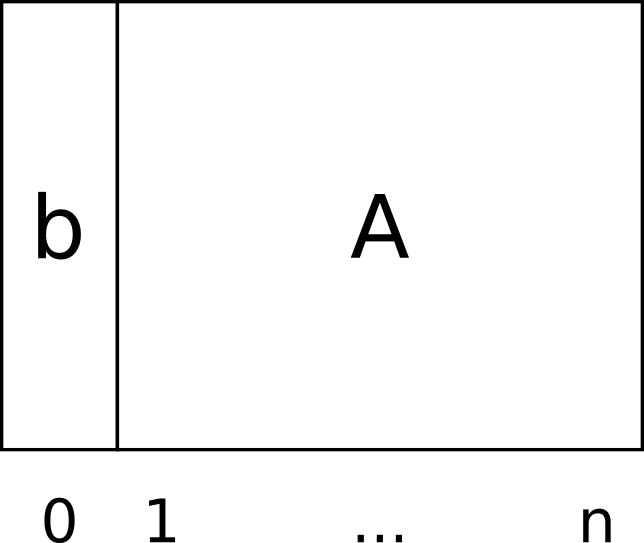
\includegraphics[width=0.3\textwidth]{images/tableau.png}
  \caption{La struttura del tableau}
  \label{tableau}
\end{figure}

\vspace{11pt}
$\blacktriangleright$ {\bf Esempio}: consideriamo il seguente sistema:

\begin{center}

  $\begin{sistema}
  x_1 + x_2 + x_3 = 2 \\
  x_1 + 3x_2 + x_4 = 3 \\
  x_1 + 4x_2 + x_3 + x_5 = 4
  \end{sistema}$

\end{center}

Il tableau ad esso corrispondente sar\`a:

\begin{center}
  
  \begin{tabular}{c|ccccc}
    & $x_1$ & $x_2$ & $x_3$ & $x_4$ & $x_5$ \\\hline
    2 & 1 & 1 & 1 & 0 & 0 \\
    3 & 1 & 3& 0 & 1& 0 \\
    4 & 1 & 4 & 1 & 0 & 1 \\
  \end{tabular}

\end{center}
$\blacktriangleleft$
\linebreak\vspace{11pt}

Noi siamo interessati a particolari tableau, quelli che presentino
nelle colonne base la matrice identit\`a (a breve vedremo il
motivo). Per ricondurci ad una soluzione del genere possiamo compiere
due operazioni che non variano la soluzione al sistema:

\begin{itemize}
\item moltiplicazione di una riga per una costante diversa da zero;
\item somma di un multiplo di una riga ad un'altra riga.
\end{itemize}

\vspace{11pt}
$\blacktriangleright$ {\bf Esempio}: riprendiamo il tableau
dell'esempio precedente.

\begin{center}

  \begin{tabular}{c|ccccc}
    & $x_1$ & $x_2$ & $x_3$ & $x_4$ & $x_5$ \\\hline
    2 & 1 & 1 & 1 & 0 & 0 \\
    3 & 1 & 3& 0 & 1& 0 \\
    4 & 1 & 4 & 1 & 0 & 1 \\
  \end{tabular}

\end{center}

Da questo possiamo ottenere, supponendo che la base sia
$\mathcal{B}=\{A_3, A_4, A_5\}$, la matrice identit\`a al suo interno
semplicemente sottraendo la riga 1 alla 3:

\begin{center}
  
  \begin{tabular}{c|ccccc}
    & $x_1$ & $x_2$ & $x_3$ & $x_4$ & $x_5$ \\\hline
    2 & 1 & 1 & 1 & 0 & 0 \\
    3 & 1 & 3& 0 & 1& 0 \\
    2 & 0 & 3 & 0 & 0 & 1 \\
  \end{tabular}

\end{center}
$\blacktriangleleft$
\linebreak\vspace{11pt}

A questo punto possiamo introdurre le due propriet\`a che ci portano a
preferire una struttura di questo tipo per il nostro tableau:

\begin{itemize}
  
\item per ogni colonna $A_j \not\in \mathcal{B}$ i coefficienti
  $y_{ij}$ richiesti dall'equazione \ref{seconda} per esprimere la
  colonna $A_j$ in funzione delle colonne di base sono  presenti nella
  colonna $j$ del tableau. Supponendo di voler esprimere $A_2$ in
  funzione delle altre colonne avremo: $A_2 = 1\cdot A_3 + 3\cdot A_4
  + 3\cdot A_5$.

\item i valori delle variabili base nella {\em SBA} corrispondente
  sono i valori presenti nella colonna 0 del tableau ($x_0 =
  (0,0,2,3,2)$).

\end{itemize}

A questo punto, considerando i vantaggi di questa struttura e
considerando che l'algoritmo del simplesso richiede che ci si muova
fra le basi, come possiamo fare a cambiar base mantenendo sempre la
struttura con una matrice identit\`a in base?

Come abbiamo imparato, il primo passo \`e quello di calcoalre
$\vartheta_{max}$. Lo possiamo calcolare facilmente vedendo il minimo
fra tutti i rapporti fra un elemento della colonna $0$ e un elemento
della colonna da far entrare in base. Nel tableau, il denominatore di
$\vartheta_{max}$ identifica il cosiddetto {\bf pivot}. Dal pivot
possiamo capire quale colonna uscir\`a dalla base: uscir\`a la colonna
che ha $1$ nella stessa posizione del pivot. Tramite le operazioni
elementari si provveder\`a poi a trasformare la colonna del pivot in
una colonna con tutti 0 e un 1 nella posizione del pivot. Sulle altre
colonne della base tali modifiche non hanno effetto.

\vspace{11pt}
$\blacktriangleright$ {\bf Esempio}: consideriamo il precedente
esempio. Calcoliamo $\vartheta_{max}$.

\begin{center}
$\vartheta_{max} = min \biggr\{ \frac{2}{1},\frac{3}{3},\frac{2}{3}
  \biggr\} = \frac{2}{3} = \frac{y_{30}}{y_{32}}$  
\end{center}

Il {\bf pivot} \`e dunque $y_{32} = 3$, l'ultimo elemento della
colonna $A_2$. Questo ci dice che dovremo inserire in base una colonna
del tipo $(0,0,1)'$, pertanto capiamo che la colonna che dovr\`a uscire
dalla base sar\`a $A_5$. A questo punto per far entrare in base la
colonna $A_5$ dobbiamo applicare delle trasformazioni elementari di
riga che ci portino ad avere $(0,0,1)'$ nella colonna 2. Le
trasformazioni necessarie sono:

\begin{itemize}

\item dividere la riga 3 per il pivot in modo da ottenere 1 al suo
  posto;

\item sottrarre ad ogni altra riga {\em i} la nuova riga del pivot
  moltiplicata per il valore attuale che si ha nella riga {\em i}
  della colonna del pivot (per ottenere 0).

\end{itemize}

Si ottiene perci\`o:

\begin{center}
  \begin{tabular}{c|ccccc}
    & $x_1$ & $x_2$ & $x_3$ & $x_4$ & $x_5$ \\\hline
    $\frac{4}{3}$ & 1 & 0 & 1 & 0 & $-\frac{1}{3}$ \\
    1 & 1 & 0& 0 & 1& -1 \\
    $\frac{2}{3}$ & 0 & 1 & 0 & 0 & $\frac{1}{3}$ \\
  \end{tabular}
\end{center}

$\blacktriangleleft$
\linebreak\vspace{11pt}

Formalmente esprimiamo il cambiamento di base ({\em pivoting}) come:
dato il tableau $[y_{ij}] (i=1,\dots,m; j=0,\dots,n)$ con base
$\beta(i)$ e pivot $y_{l_j}x$, il nuovo tableau $[\tilde{y}_{ij}]$ \`e
dato da:

\begin{itemize}
\item $\tilde{y}_{lq} = \frac{y_{lq}}{y_{lj}} (q = 0,\dots,n)$;
\item $\tilde{y}_{iq} = y_{iq} - \tilde{y}_{lq}y_{ij} (i=1,\dots,m,
  i\neq l; q=0,\dots,n)$
\end{itemize}

e la nuova base \`e: $\tilde{\mathcal{\beta}}(i) = 
\begin{sistema}
\beta (i),\phantom{aaa} i\neq l;\\
j,\phantom{aaa} i=l;
\end{sistema}
$

\section{Pivoting e valore della soluzione}

Per scegliere quale colonna fare entrare in base, conviene valutarne
l'effetto sulla funzione obiettivo. 

Indichiamo con $\mathcal{B}$ la base attuale e con $x_0' = (y_{10},
y_{20}, \dots, y_{m0}, 0, \dots, 0)$ la SBA ad essa corrispondente. Il
valore della soluzione \`e:

\begin{center}
$z(\mathcal{B}) = \sum_{i=1}^m y_{i0}c_{\beta(i)}$ 
\end{center}

dove, lo ricordiamo, $y_{10}$ sono le componenti di $x_0$ appartenenti
alla base mentre $c_{\beta(i)}$ sono le variabili della funzione costo
relative alle variabili in base.

Adesso riprendiamo la relazione \ref{theta}:

\begin{center}
$\sum\limits_{i=1}^m (y_{i0} - \vartheta y_{ij}) A_{\beta(i)} +
  \vartheta A_j = b\phantom{aaa}\forall A_j \not\in \mathcal{B} $
\end{center}

Poniamo $\vartheta=1$, cio\`e facciamo entrare in base una unit\`a di
$x_j$. In questo caso il costo diventa:

\begin{center}
$\tilde{z}(\mathcal{B} =
\sum\limits_{i=1}^m(y_{i0}-y_){ij})c_{\beta(i)} + 1 \cdot c_j =
z(\mathcal{B}) - \sum\limits_{i=1}^m y_{ij} c_{\beta(i)} + c_j$
\end{center}

cio\`e per ogni unit\`a che entra in base il costo varia di:

\begin{center}
$c_j - \sum\limits_{i=1}^m y_{ij} c_{\beta(i)}$
\end{center}

Questo valore viene detto {\bf costo relativo} della colonna {\em j},
lo indichiamo con:

\begin{center}
$\bar{c}_j = c_j - \sum\limits_{i=1}^m y_{ij}
c_{\beta(i)} = c_j - z_j$
\end{center}

Indipendentemente dal valore di $\vartheta_{max}$ dovremo far entrare
in base una colonna $A_j$ solo se $\bar{c}_j < 0$, cio\`e se il costo
passando dalla base $\mathcal{B}$ alla nuova base con $A_j$
diminuisce.

Come ricavare questa informazione dal tableau? Dal momento che il
tableau rappresenta delle equazioni, introduciamo una nuova variabile
($-z$). Tale variabile corrisponde all'opposto del valore della
funzione obiettivo. Risulta pertanto:

\begin{center}
$0 = \sum\limits{i=1}{n} c_jx_j + (-z)$  
\end{center}

Questa equazione la inseriremo nella riga 0 del tableau ottenendo
ci\`o che vediamo in figura \ref{tableau2}.

\begin{figure}[h!]
  \centering
  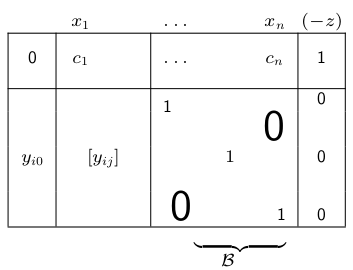
\includegraphics[width=0.5\textwidth]{images/tableau2.png}
  \caption{figura esemplificativa}
  \label{tableau2}
\end{figure}

A questo punto \`e per\`o necessario compiere quelle operazioni che ci
faranno avere 0 al costo delle variabili in base. Queste operazioni
consistono nel moltiplicare ogni riga {\em i} per il valore del costo
$c_{\beta(i)}$ che vogliamo annullare e poi sottrarle alla riga 0.

Otterremmo il tableau di figura \ref{tableau3}

\begin{figure}[h!]
  \centering
  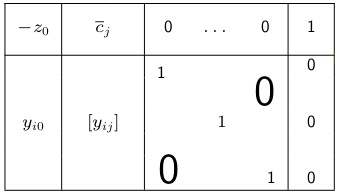
\includegraphics[width=0.5\textwidth]{images/tableau3.png}
  \caption{figura esemplificativa}
  \label{tableau3}
\end{figure}

Da questo tableau ricaviamo il costo di ogni colonna fuori base. In
realt\`a l'ultima colonna che vediamo \`e stata aggiunta per far si
che la matrice identit\`a abbia ordine {\em n+1}, tuttavia dal momento
che rimane sempre uguale non viene solitamente considerata.

\section{Criterio di ottimalit\`a}

{\bf Teorema:} se $\hat{c}_j \geq 0 \forall j$ allora la soluzione
corrente $x_0$ \`e ottimale.

\vspace{11pt}
$\square$ {\bf Dimostrazione}: l'equazione della riga 0 del tableau
attuale \`e:

\begin{center}
$z = z_0 + \sum\limits_{A_j \not\in \mathcal{B}} \hat{c}_jx_j$  
\end{center}

e ci dice che il valore {\em z} di qualunque soluzione (inclusa quella
ottima) \`e dato dal valore $z_0$ della soluzione attuale pi\`u una
combinazione lineare $\sum\limits_{A_j \not\in \mathcal{B}}
\hat{c}_jx_j$ degli attuali cost irelativi.

Poich\'e siamo vincolatia soluzioni nelle quali $x_j \geq 0 \forall j$,
si ha che, se $\hat{c} \geq 0 \forall A_j \not \in \mathcal{B}$,
qualunque soluzione ammissibile pu\`o solo avere un valore maggiore o
uguale a quello della soluzione attuale. $\blacksquare$
\vspace{11pt}

\section{Prima versione dell'algoritmo del simplesso}
\small
\begin{center}
\begin{tabular}{||l||}
\hline\hline
{\bf procedure SIMPLEX}:\\
begin\\
\phantom{aaa}optimal := unbounded := false;\\
\phantom{aaa}{\bf while} optimal = false {\bf and} unbounded = false {\bf do}\\
\phantom{aaaaaa}{\bf if} $c_j \geq 0 \forall j$ {\bf then} optimal = true\\
\phantom{aaaaaa}{\bf else}\\
\phantom{aaaaaaaaa}{\bf begin}\\
\phantom{aaaaaaaaaaaa}choose any j such that $\hat{c}_j < 0$;\\
\phantom{aaaaaaaaaaaa}{\bf if} $y_{ij} \leq 0 \forall i > 0$ {\bf then} unbounded := true\\
\phantom{aaaaaaaaaaaa}{\bf else} $\vartheta_0 := min_{i:y_{ij}>0}
\frac{y_{i0}}{y_{ij}} = \frac{y_{l0}}{y_lj}$ and pivot on $y_{lj}$\\
\phantom{aaa}end\\
end.\\
\hline\hline
\end{tabular}
\end{center}
\normalsize

Se non si entrano basi degeneri, il valore della soluzione decresce ad
ogni iterazione, il che implica che ogni SBA generata \`e diversa
dalle precedenti. Quindi, sotto le ipotesi restrittive fatte, il
metodo converge.

Quella considerata non pu\`o che essere solo la prima versione
dell'algoritmo del simplesso in quanto non abbiamo considerato le basi
degeneri ed in quanto non abbiamo un metodo per costruire un tableau
con una base iniziale.

\section{Degenerazione ciclante}

Dimostriamo con un esempio che le basi degeneri possono causare dei
loop. Assumiamo come regole di pivoting:

\begin{itemize}
  
\item la variabile con il costo $\hat{c}_j$ "pi\`u negativo" entra in
  base;
\item in caso di parit\`a la variabile con l'indice minore lascia la
  base.

\end{itemize}

L'esempio \`e visibile in figura \ref{td}.  Come possiamo vedere
giungiamo ad un loop in quanto siamo ritornati alla situazione di
partenza.

\begin{figure}[h!]
  \centering
  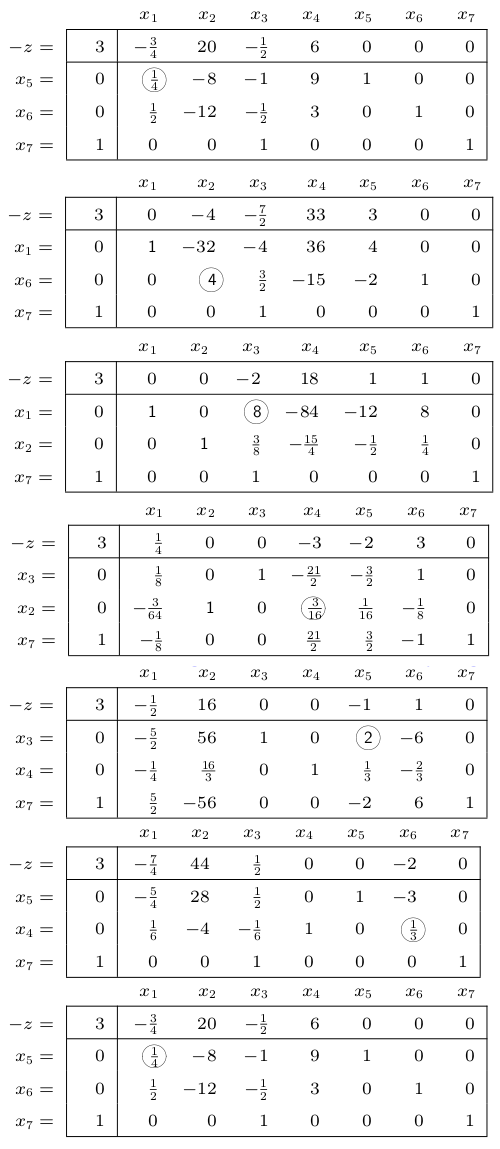
\includegraphics[width=0.55\textwidth]{images/td.png}
  \caption{Basi degeneri e looping}
  \label{td}
\end{figure}

\section{Regole di pivoting}

Nel momento in cui dobbiamo effettuare il pivoting dobbiamo prendere
due decisioni:

\begin{itemize}

\item quale colonne, fra quelle a costo $\hat{c}_j < 0$, far entrare
  in base;

\item cosa fare in caso si abbiano righe che producano lo stesso
  $\vartheta$.

\end{itemize}

Per scegliere la colonna da far entrare in base possiamo applicare
vari metodi:

\begin{itemize}
  
\item possiamo scegliere la colonna $A_j$ con il costo $\hat{c}_j$
  negativo minore fra tutti (\`e detta {\bf Regola di Dantzig} ed \`e
  la pi\`u efficiente);

\item possiamo scegliere la colonna $A_j$ che produce il maggior
  decremento del costo (computazionalmente molto complesso);

\item possiamo applicare la {\bf regola di Bland} che afferma che
  entra in base la colonna $A_j$ con il pi\`u piccolo $j$. \`E provato
  che questo metodo ci salva dai loop, tuttavia converge molto pi\`u
  lentamente. In caso di parit\`a dei valori $\vartheta$ si sceglie di
  far uscire dalla base la colonna con indice $j$ minore.

\end{itemize}


\section{Determinazione di una SBA iniziale}

Da questo punto in poi saremo a conoscenza dell'algoritmo completo, un
algoritmo composto da due fasi: la {\em fase 1} in cui si determina
una SBA iniziale e, se questa esiste, si passa alla {\em fase 2} che
\`e costituita dall'algoritmo del simplesso per risolvere il problema.

Vediamo dunque come si svolge la fase uno.

\begin{enumerate}
  
\item Se esistono termini noti $b_i$ negativi si cambia segno alle
  equazioni corrispondenti.

\item Si aggiungono {\em m} variabili artificiali $x_i^a \geq 0$
  (cio\`e tante quante sono le righe del tableau) con coeffciente 1 e
  si somma ad ogni equazione {\em i} il termine $x_i^a (i=1,\dots,m)$
  (in parole povere ad ogni equazione si aggiunge il termine $+ 1
  \cdot x_i$ nella corrispondente equazione {\em i} e quindi si
  ottiene una matrice identit\`a affiancata al tableau originale). A
  questo proposito, se il sistema presenta gi\`a alcune colonne della
  matrice identit\`a \`e possibile introdurre meno di {\em m} colonne,
  ma solo quelle mancanti per completare la matrice {\em I}. Il nuovo
  sistema ha una SBA ottima, tuttavia non \`e una soluzione
  ammissibile per il sistema $Ax=b$ originale, dato che ottenuta con
  delle variabili artificiali.

\item A questo punto si minimizza tramite il {\bf simplesso} la
  funzione obiettivo artificiale, cio\`e:

  \begin{center}
    $min \zeta = \sum\limits_{i=1}^m x_i^a$
  \end{center}

  Dobbiamo in pratica eliminare, mediante una sequenza di pivoting,
  l'uso delle variabili artificiali per soddisfare i vincoli. Se
  questo sistema possiede una soluzione con valore $\zeta = 0$ allora
  il sistema originale ammetter\`a soluzione, se $\zeta > 0$ allora il
  problema originale non ammette alcuna soluzione (\`e violata
  l'assunzione 2 che abbiamo fatto in precedenza) e l'esecuzione
  termina.

  In particolare per\`o, se $\zeta = 0$ possiamo avere pi\`u casi:
  
  \begin{itemize}
  \item se le variabili artificiali sono fuori base, allora il tableau
    ha una corrispondenza con le variabili vere; si possono quindi
    eliminare le variabili artificiali (che non essendo in base
    varranno 0), si pu\`o sostituire la funzione obiettivo artificiale
    con la vera funzione obiettivo, azzerare i costi corrispondenti
    alla base e risolvere tramite l'algoritmo del simplesso;

  \item se almeno una variabile artificiale \`e in base occorrono
    altre considerazioni che vedremo pi\`u in l\`a.
  \end{itemize}

\end{enumerate}

\vspace{11pt}
$\blacktriangleright$ {\bf Esempio}: risolviamo usando la regola di
Bland il problema:

\vspace{11pt}
\begin{center}
  \begin{tabular}{l}
    $\min z = x_1 + x_3$\\
    $\phantom{min}x_1 + 2x_2 \leq 5 \rightarrow x_1 + 2x_2 + s_1 = 5$\\
    $\phantom{min}x_2 + 2x_3 = 6$\\
    $\phantom{min}x_1, x_2, x_3 \geq 0 \rightarrow x_1, x_2, x_3, s_1
    \geq 0$\\
  \end{tabular}
\end{center}
\vspace{11pt}

In figura \ref{cap4fase1} \`e possibile osservare la fase 1
dell'algoritmo del simplesso.

\begin{figure}[h!]
  \centering
  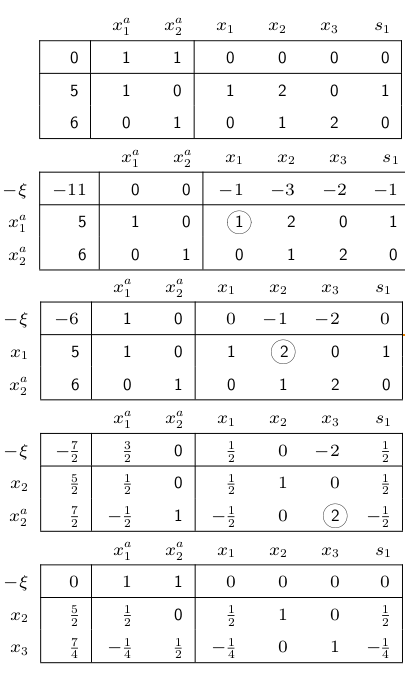
\includegraphics[width=0.6\textwidth]{images/cap4fase1.png}
  \caption{Fase 1}
  \label{cap4fase1}
\end{figure}


Nella fase 1 sono state aggiunte due variabili artificiali, tuttavia
avremmo potuto introdurne anche soltanto una dato che la colonna
$x_1^a$ ha gi\`a la forma di una colonna della matrice identit\`a.


La fase 2 \`e in figura \ref{cap4fase2}. In questa fase le colonne
delle variabili artificiali potrebbero tranquillamente essere
eliminate. Se si sceglie di non eliminarle, in fase di pivot si devono
considerare soltanto le variabili vere.

\begin{figure}[h!]
  \centering
  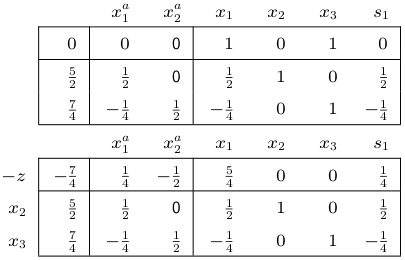
\includegraphics[width=0.6\textwidth]{images/cap4fase2.png}
  \caption{Fase 2}
  \label{cap4fase2}
\end{figure}

Ricaviamo la soluzione ottima $x' = (0, \frac{5}{2}, \frac{7}{4})$ di
valore $z = \frac{7}{4}$. $\blacktriangleleft$
\vspace{11pt}

\vspace{11pt}
$\blacktriangleright$ {\bf Esempio}: consideriamo ora il problema:

\vspace{11pt}
\begin{center}
  \begin{tabular}{l}
    $\min z = x_1 + x_3$\\
    $\phantom{min}x_1  2x_2 \leq -5\phantom{a}\rightarrow\phantom{a}x_1 + 2x_2 + s_1 = -5\phantom{a}\rightarrow\phantom{a} -x_1 - 2x_2 -s_1 = 5$\\
    $\phantom{min}x_2 + 2x_3 = 6$\\
    $\phantom{min}x_1, x_2, x_3 \geq 0 \rightarrow x_1,x_2,x_3,s_1 \geq 0$\\
  \end{tabular}
\end{center}
\vspace{11pt}

\begin{figure}[h!]
  \centering
  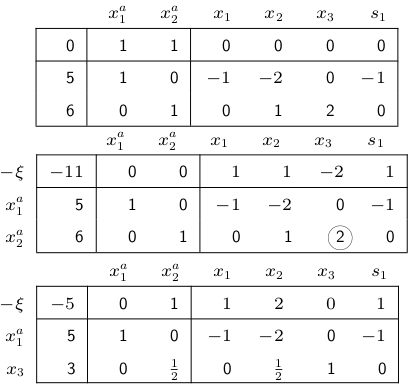
\includegraphics[width=0.6\textwidth]{images/cap4fase1es2.png}
  \caption{Fase 1}
  \label{cap4fase1es2}
\end{figure}

In questo caso, come possiamo vedere in figura \ref{cap4fase1es2} il
tableau ottimo della fase 1 d\`a una soluzione non nulla per cui il
problema non ha soluzioni ammissibili. $\blacktriangleleft$
\vspace{11pt}

\vspace{11pt}
$\blacktriangleright$ {\bf Esempio}: prendiamo ora in esame il
seguente problema:

\vspace{11pt}
\begin{center}
  \begin{tabular}{l}
    $\min z = x_1 + x_2 + 10x_3$\\
    $\phantom{min}x_2  4x_3 =2$\\
    $\phantom{min}2x_1 - x_2 + 6x_3 = -2\phantom{a}\rightarrow\phantom{m} -2x_1 + x_2 -
    6x_3 = 2$\\
    $\phantom{min}x_1, x_2, x_3 \geq 0$\\
  \end{tabular}
\end{center}
\vspace{11pt}

Come al solito procediamo a svolgere al fase 1 (Figura
\ref{cap4fase1es3}).

\begin{figure}[h!]
  \centering
  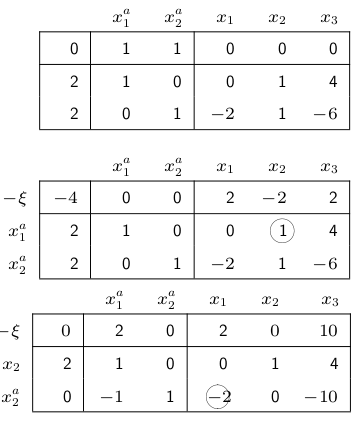
\includegraphics[width=0.6\textwidth]{images/cap4fase1es3.png}
  \caption{Fase 1}
  \label{cap4fase1es3}
\end{figure}

In questo caso la soluzione della fase 1 ha valore nullo, ma la
variabile artificiale $x_2^a$ \`e in base per cui non possediamo una
base sulle variabili vere. 

Effettuiamo un pivoting apposta per ottenere una colonna vera in base
e procedendo poi con la fase 2 arriveremo alla soluzione $x' =
(0,2,0)$ di valore $z = 2$. Tutto ci\`o \`e mostrato in figura
\ref{cap4fase2es3}. 

\begin{figure}[h!]
  \centering
  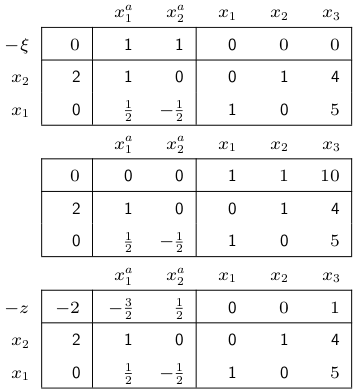
\includegraphics[width=0.6\textwidth]{images/cap4fase2es3.png}
  \caption{Fase 2}
  \label{cap4fase2es3}
\end{figure}

In questo esempio, come detto avevamo la soluzione della fase 1 pari a
0, ma con una variabile artificale in base (con valore 0). Per ogni
riga {\em i} con tale propriet\`a si effettua un pivoting con un pivot
$y_{ij} \neq 0$ corrispondente ad una variabile non artificiale. Se si
riesce a portare ogni variabile artificiale fuori base si prosegue con
la fase 2, altrimenti vuol dire che esiste almeno una variabile
artificiale $x_i^a$ in base tale che $y_{ij} = 0$ per ogni variabile
non artificiale. Ci\`o implica che a seguito di una sequenza di
operazioni elementari di riga, la riga {\em i} rappresenta ora
l'equazione $(0,\dots,0)'x = 0$. Questo vuol dire che la matrice {\em
  A} non \`e di rango {\em m} e dunque che \`e violata l'assunzione 1
fatta in precedenza. Cosa si fa in tale situazione? Per ogni $x_i^a$
in base tale che $y_{ij} = 0$ per ogni variabile non artificiale, si
elimina la riga $i$ e si esegue la fase 2 con una base di dimensione
inferiore.  $\blacktriangleleft$
\vspace{11pt}

\section{Algoritmo del simplesso - versione completa}

\small
\vspace{11pt}
\begin{center}
\begin{tabular}{||l||}
\hline\hline
{\bf procedure TWO PHASE}:\\
{\bf begin}\\
\phantom{aa}impossible := redundant := false;\\
\phantom{aa}{\bf for each} $b_i < 0$ {\bf do} multiply the {\em i}th equation by -1;\\
\phantom{aa}{\bf for} i:=1 {\bf to} m {\bf do} add the term $x_i^a$ to the {\em i}th equation;\\
\phantom{aa}inserisci nella riga 0 la funzione obiettivo $\zeta = \sum\limits_{i=1}^m x_i^a$\\
\phantom{aa}{\bf for} i := 1 {\bf to} m {\bf do} riga 0 := riga 0 - riga i;\\
\phantom{aa}{\bf call SIMPLEX};\\
\phantom{aa}\phantom{aa}\phantom{aa}{\bf if} $\zeta^*$ (= solution value) > 0 {\bf then} impossible := {\bf true} ({\bf comm.}: Ass.2 violated)\\ 
\phantom{aa}{\bf else}\\
\phantom{aaaa}{\bf begin}\\
\phantom{aaaaaa}{\bf for each} artificial variable $x_i^a$ in base {\bf do}\\
\phantom{aaaaaaaa}{\bf if} $\exists y_{ij} \ne 0$ : $x_j$ is non-artificial {\bf then} perform a pivoting on $y_{ij}$\\
\phantom{aaaaaaaa}{\bf else begin}\\
\phantom{aaaaaaaaelsea}redundant := true ({\bf comm.}: Ass.1 violated);\\
\phantom{aaaaaaaaelsea}eliminate row i, and set m := m - 1\\
\phantom{aaaaaaaaelsea}{\bf end};\\
\phantom{aaaaaa}insert the original objective function in row 0;\\
\phantom{aaaaaa}{\bf for} i := 1 {\bf to} m {\bf do} row 0 := row 0 - $c_{\beta(i)} \cdot$ (row {\em i});\\
\phantom{aaaaaa}{\bf call SIMPLEX}\\
\phantom{aaaa}{\bf end}\\
{\bf end.}\\\hline\hline
\end{tabular}
\end{center}
\vspace{11pt}
\normalsize

\section{Interpretazione geometrica dell'algoritmo del simplesso}

L'algoritmo del siplesso esplora una sequenza di {\bf vertici
  adiacenti}. Due vertici di un politopo si dicono adiacenti se sono
connessi da uno spigolo.

{\bf Teorema:} dato il politopo {\em P} definito dai vincoli di un
problema di programmazione lineare, condizione necessaria e
sufficiente perch\'e un segmento $[\bar{x},\bar{y}] \in P$ sia uno
spigolo \`e che i corrispondenti vettori {\em x}, {\em y} siano SBA
adiacenti dell'ILP. ($[\bar{x},\bar{x}]$) \`e considerato un segmento
di lunghezza nulla.

La programmazione lineare \`e un caso particolare di programmazione
convessa per cui se un punto {\em x} \`e un ottimo locale rispetto ad
un intorno euclideo {\em E(x)} comunque piccolo, esso \`e anche un
ottimo globale.

Un intorno euclideo comunque piccolo \`e costituito per\`o da un
numero infinito di punti, mentre noi potremmo considerare anche un
numero finito e piccolo di punti. Il criterio di ottimalit\`a della
programmazione lineare, infatti, ha evidenziato un intorno pi\`u
importante: se un vertice {\em x} \`e un ottimo locale rispetto
all'insieme $A(x)$ dei vertici adiacenti, esso \`e anche un ottimo
globale. Proprio perch\'e ci si muove fra pochi elementi (il numero di
colonne fuori base candidate ad entrare in base \`e limitato a $n-m$)
l'algoritmo del simplesso \`e molto efficiente.

\begin{figure}[h!]
  \centering
  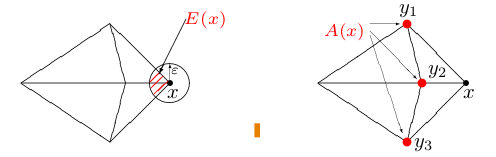
\includegraphics[width=0.8\textwidth]{images/cap4fig42.png}
  \caption{Intorni euclidei ed intorni discreti}
  \label{cap4fig42}
\end{figure}

Nel caso di problemi non lineari, anche se la regione ammissibile \`e
prodotta da vincoli lineari, abiamo il problema di dover cercare la
soluzione {\bf all'interno del politopo}, dunque di dover analizzare
un numero infinito di punti. 

Un altro caso ancora \`e quello in cui la funzione obiettivo \`e
lineare, ma i vincoli non lo sono. In questo caso la soluzione ottima
pu\`o trovarsi in {\bf un punto qualunque del confine} del politopo.

In entrambi i casi dunque la soluzione va cercata analizzando un
numero infinito di punti!

\end{document}
